\documentclass[11pt]{article}
\usepackage[margin=1in]{geometry}
\usepackage{amsmath,amssymb,amsfonts}
\usepackage{graphicx}
\usepackage{booktabs}
\usepackage{multirow}
\usepackage{array}
\usepackage{url}
\usepackage{cite}
\usepackage{caption}
\captionsetup{font=small,labelfont=bf}
\graphicspath{{../paper/figures/}{../paper/}}
\setlength{\parskip}{2pt}

\title{\textbf{Version Migration as a Correlated Shock: Model Updates as an Unmanaged Risk Channel in LLM-Based Financial Systems}%
\thanks{This work received no specific grant from any funding agency in the public, commercial, or not-for-profit sectors. Corresponding author: Robin Chawla (robin.chawla.cse14@iitbhu.ac.in).}}
\author{Samir Chincholikar\thanks{Independent Researcher. Email: samir.chincholikar@gmail.com; ORCID 0009-0007-2779-3492.}
\and Robin Chawla\thanks{Independent Researcher. Email: robin.chawla.cse14@iitbhu.ac.in; ORCID 0009-0007-2807-3948.}}
\date{Preprint --- August 2026. This is a preprint and has not been peer reviewed.}

\begin{document}
\maketitle

\begin{abstract}
Financial institutions increasingly deploy large language models (LLMs) within credit and other decision-support workflows. However, vendor-driven model updates can alter behavior even when an institution holds its prompts, inputs, and downstream processes fixed. We quantify the decision instability associated with two prespecified model-version transitions: an OpenAI efficient-model update and a Google Gemini Flash update. Across both transitions, the experiment covers 100 companies, 12 analysis dates, and three replicates per version, producing 14,400 model calls. Identical inputs and matched per-cell seeds hold sampling conditions fixed, and within-version replicate disagreement provides an empirical noise floor. The primary endpoint is the excess cross-version flip rate above this floor. For the OpenAI migration, the cross-version disagreement rate exceeds the within-version noise floor by 11.2 percentage points (95\% CI: 7.7--15.0); for the Gemini migration this excess is 38.1 percentage points (95\% CI: 30.3--45.8). A prevalence--churn decomposition shows that the OpenAI update primarily reconsiders individual companies and shifts decisions toward greater severity, while the Gemini update produces a broad distributional shift toward the SAFE category. Neither migration shows clear improvement among observations whose labels change; the Gemini successor also shows lower aggregate class-balanced performance. Vendor version migration can therefore create material, directionally unpredictable decision discontinuities within otherwise unchanged LLM pipelines. We propose a pre-migration parallel-run control that measures excess flip rate, label-distribution shift, per-company churn, and directional drift before production cutover. The findings provide controlled evidence of deployment-level migration risk; broader cross-task and cross-institution effects remain for future study.
\end{abstract}

\noindent\textbf{Keywords:} Algorithmic monoculture, credit risk, financial artificial intelligence, large language models, model drift, model risk management, model version migration, reproducible evaluation, third-party model risk

\medskip

\section{Introduction}
Large language models (LLMs) are increasingly being integrated into financial decision-support workflows~\cite{bloomberggpt,finbert} such as credit screening, counterparty assessment, disclosure review, and operational triage. In these applications, model outputs can feed into downstream classifications, escalation decisions, and review priorities. However, many LLMs are accessed via application programming interfaces (APIs) provided by third parties, in which case the provider determines the versions and availability of the underlying models. This differs from conventional models developed within an institution and governed by existing model-risk processes~\cite{sr117,sr2602}. When an existing model version is deprecated or replaced, institutions may therefore be forced to migrate to a successor version even if their prompts, data, application logic, and downstream processes remain unchanged.

These migrations are a distinct form of model-change risk. A successor version could act like its predecessor, with little impact on operations. But the same inputs can also lead to materially different decisions depending on changes in training data, architecture, optimization, or alignment~\cite{muscle,underspec,bommasani}. Just because a provider marks a version as the recommended replacement does not mean that it is behaviorally equivalent to its predecessor~\cite{wei}. The magnitude, direction, and structure of any resulting decision changes thus have to be empirically measured under controlled input and sampling conditions.

There are two main measurement challenges in model update evaluation. First, repeated calls to the same model version can yield different outputs because of residual sampling variability. Therefore, a simple before-and-after disagreement rate may mistakenly attribute normal within-version variation to the migration itself. Second, the aggregate flip rate does not capture how decisions are changing. A successor version may change the overall distribution of labels across the portfolio being evaluated, or it may move individual companies in offsetting directions with little change in the aggregate distribution. These two types of changes have different operational and governance implications and should therefore be measured separately.

This study assesses two vendor model migrations using a controlled financial classification task. For each migration, the incumbent and successor versions receive identical dated financial information and matched cell-level sampling seeds. We estimate the ordinary noise floor using within-version replicate disagreement and measure the cross-version flip rate in excess of this baseline as the primary endpoint. We further decompose the observed migration-induced changes into a marginal label-distribution shift and company-level churn, examine directional movement between credit-health categories, and perform a secondary analysis comparing both versions against a deterministic, rule-based Altman $Z''$-based financial-health reference~\cite{altman,altman_em}.

This paper focuses on migration risk at the deployment level: the possibility that a provider-controlled update materially changes decisions within an otherwise unchanged LLM pipeline. When a particular model version is used by multiple deployments, they may undergo the same vendor-initiated change around the same time, resulting in synchronized changes across these systems~\cite{kim,systemic,homog,esrb}. We term this common upstream version change and its potential to affect multiple deployments a ``correlated shock.'' It does not imply an empirical measurement of cross-institutional correlations or realized effects at the market level. Instead, this research provides controlled evidence that the underlying mechanism for such a shared decision shock exists and is quantifiable.

The principal contributions of this study are as follows:
\begin{enumerate}
\item \textbf{Controlled measurement of migration-induced decision instability:} We quantify the decision instability associated with two vendor model migrations using an explicit within-version noise floor to separate migration-induced disagreement from normal sampling variability.
\item \textbf{Mechanism-level decomposition:} We decompose migration-induced decision changes into marginal label-distribution shifts and company-level churn, and use chance-corrected agreement and directional-drift measures to further characterize the structure of these changes.
\item \textbf{Outcome linkage:} We evaluate whether the decisions changed by each model migration are associated with improved classification performance against a deterministic, rule-based financial-health reference.
\item \textbf{Governance application:} We convert the empirical measurements into a pre-migration parallel-run control that can identify material decision changes before production cutover.
\item \textbf{Reproducible research artifact:} We release frozen inputs, exact model-version identifiers, matched seeds, raw model responses, preregistration materials, and a deterministic analysis pipeline that reproduces the reported results.
\end{enumerate}

\section{Related Work}
\subsection{Model-Update Regression in General Machine Learning}
Even if the task inputs and downstream decision rules remain the same, model updates can alter predictions. In prior work, such instance-level regressions are referred to as negative flips, where a successor model overturns a previously correct or stable prediction. Work on LLM evolution has tackled this problem by proposing compatibility mechanisms to reduce regressions across model versions~\cite{muscle}, building on prior work on regression-free model updates~\cite{pctrain}. Related work in concept drift research distinguishes true changes in model behavior from normal within-model variability~\cite{gama}, while standardized model-evaluation frameworks emphasize the importance of assessing successor models before deployment~\cite{helm}. Task underspecification studies also demonstrate that seemingly fixed prompts can provide significant behavioral freedom to the underlying model~\cite{underspec,sclar}, allowing version updates to affect responses along dimensions that are not explicitly constrained by the prompt.

Previous work mostly casts model-update regression as a problem of model performance, compatibility, or deployment engineering. The question addressed in the present study is a complementary one: how much does a vendor-directed version migration change categorical financial decisions after accounting for normal within-version response variability? Rather than looking only at the improvement or deterioration of individual predictions, we also measure the overall decision discontinuity, its directional structure, and the changes in the portfolio of classifications. This extends model-update research from instance-level compatibility to the operational risk arising from a provider-controlled migration that affects an otherwise unchanged financial decision pipeline.

\subsection{Algorithmic Monoculture and Systemic Risk in Finance}
More and more studies investigate whether widespread reliance on similar artificial intelligence systems can lead to correlated behavior across financial institutions and markets. Shared foundation models, common training data, and similar optimization objectives may cause otherwise independent users to make increasingly aligned decisions, reducing effective model diversity and increasing exposure to common failures~\cite{monoculture,kim}. Related studies have linked this convergence to algorithmic herding, concentration risk, and broader forms of systemic fragility~\cite{systemic,homog}. Supervisory research has also begun to identify AI homogenization as a possible source of correlated risk in the financial system~\cite{esrb,fsb}.

Most of the existing work has taken a conceptual or market-level approach to the problem of correlated trading and decision behavior. However, less direct empirical evidence exists on how a common external change might simultaneously influence decisions across deployed systems. One such mechanism is a vendor-managed model-version migration, where several deployments using the same model version can be exposed to the same successor and thus undergo a synchronized behavioral change. In this paper, we measure the effect of two vendor migrations on credit-health classifications under identical inputs and thus assess this mechanism at the decision level.

This analysis does not estimate realized systemic effects or cross-institutional losses. Instead, it identifies a mechanism through which deployments based on the same model version could experience a shared change in behavior. This evidence at the decision level contributes to the existing systemic-risk literature by linking broader concerns about model concentration to a measurable operational event in an LLM-based financial workflow.

\subsection{Agreement, Prevalence, and the Kappa Paradox}
Chance-corrected measures of agreement between an incumbent and successor model include Cohen's $\kappa$~\cite{cohen}, Scott's $\pi$~\cite{scott}, and Gwet's AC1~\cite{gwet}, with Fleiss' $\kappa$ providing a generalization to multiple raters~\cite{fleiss}. In this study, we treat the incumbent and successor model versions as paired raters that assign one of three credit-health labels (SAFE, WATCH, or DISTRESS) to the same company-date-replicate cells. These measures capture the extent to which the two versions agree in their classifications beyond the agreement expected from their marginal label distributions.

If category prevalence is very uneven, or if the prevalence shifts substantially between model versions, relying on a single agreement statistic can be misleading. Cohen's $\kappa$ and related statistics can be low even in the presence of high observed agreement, a phenomenon often called the $\kappa$ paradox~\cite{feinstein}. Gwet's AC1 is less sensitive to this prevalence effect, while Scott's $\pi$ is an alternative chance-corrected measure based on a different formulation of expected agreement. We report all three measures to evaluate whether the observed migration effect persists under different treatments of marginal label imbalance.

Agreement statistics alone, however, do not explain how the portfolio of decisions changes under a model migration. Low agreement across versions may result from a large shift in label prevalence, from offsetting company-level reclassifications that leave the aggregate label distribution largely unchanged, or from both. We therefore supplement the agreement measures with a prevalence--churn decomposition. The marginal component is the minimum proportion of observations that must change to produce the label distribution of the successor version, while the remaining churn component captures company-level reclassifications that cancel out in the aggregate.

These measures together capture three related but distinct aspects of model migration: consistency across versions, changes in the distribution of credit-health categories, and reclassification of individual firms. This provides a more informative picture of migration behavior than a raw flip rate or a single chance-corrected agreement statistic alone.

\subsection{Model Risk Management and Generative AI}
Model-risk management frameworks emphasize validation, ongoing monitoring, change control, documentation, effective challenge, and institutional accountability, including for third-party models. Historically, SR 11-7 has been the benchmark for these expectations in the United States, but its model lifecycle typically assumes that an institution can identify when a model has changed and initiate a review before the modified model is put into production~\cite{sr117}.

This assumption is complicated by vendor-hosted LLMs, where model versions may be updated, replaced, or deprecated on the provider's schedule. Hence, a migration can change model behavior even as an institution maintains its prompts, inputs, application logic, and downstream controls. Recent work has proposed broader governance frameworks for generative and agentic AI~\cite{mrm}, but the present study focuses on a narrower empirical problem: decision discontinuity caused specifically by vendor-directed model-version migration. To measure this risk, we use paired version testing, a within-version noise floor, and measures of excess disagreement, distributional shift, churn, and directional drift. The corresponding governance implications and proposed control are developed in Section~\ref{sec:gov}.

\subsection{Reproducibility and Preregistration}
Empirical LLM evaluations are sensitive to model versions, prompts, sampling settings, data selection, exclusion rules, and statistical choices~\cite{simmons}, and proprietary endpoints may change, making exact retrospective replay difficult or impossible. We therefore specify the migration pairs, evaluation grid, prompt, seeds, endpoints, reference-label procedure, and decision rule before confirmatory data collection~\cite{nosek}; assign the frozen protocol a cryptographic hash; preserve immutable call-level responses and configurations; and reproduce all reported results through a seeded, build-validated analysis pipeline~\cite{pineau}. The empirical record of the experiment is the archived responses, not future replays of the API. Full procedural details are provided in Section~\ref{subsec:freeze} and the Data and Code Availability statement.

\section{Problem Formulation and Metrics}
\subsection{Task and Unit of Analysis}
For each vendor migration, let $v_{\mathrm{old}}$ denote the incumbent model version and $v_{\mathrm{new}}$ its designated successor. The unit of analysis is a matched company--date--replicate cell,
\begin{equation}
s=(j,t,r),
\end{equation}
where $j$ identifies the company, $t$ the analysis date, and $r$ the replicate. Each model version receives the same company information for the same cell and independently assigns one credit-health category,
\begin{equation}
y_{v,s}\in\{\text{SAFE},\text{WATCH},\text{DISTRESS}\}.
\end{equation}
Each response is returned in a fixed JSON schema containing the assigned categorical label, a self-reported conviction score, and a free-text rationale. In the analysis presented here, only the categorical label is used.

The experimental comparison uses a paired design. For every valid cell, the incumbent and successor versions are evaluated using identical financial inputs, prompt structure, inference settings, and matched cell-level seeds. Model version is thus the main experimental factor that differs between the two observations in each pair.

The primary estimand is not whether either version produces the correct financial classification. Instead, it is how much replacing $v_{\mathrm{old}}$ with $v_{\mathrm{new}}$ changes the categorical decision of an otherwise unchanged pipeline. Reference labels are introduced separately for the secondary accuracy analysis and are not required to estimate the decision instability induced by migration.

\subsection{Flip Rate and the Within-Version Noise Floor}
\label{subsec:noisefloor}
A naive comparison between $v_{\mathrm{old}}$ and $v_{\mathrm{new}}$ can overstate the apparent instability due to migration, because multiple calls to the same model version may produce different labels given the same input. We therefore separate ordinary within-version variability from the additional disagreement introduced by the version change.

For version $v$, the within-version flip rate is defined as the proportion of replicate pairs for the same company and analysis date that return different categorical labels:
\begin{equation}
F_{\mathrm{within},v} = \Pr\!\left( y_{v,j,t,r_1}\neq y_{v,j,t,r_2} \right), \qquad r_1\neq r_2.
\end{equation}
Concretely, with three replicates per cell each cell contributes three unordered replicate pairs; $F_{\mathrm{within},v}$ is the fraction of all such within-cell replicate pairs, pooled across cells, that disagree. The pooled within-version noise floor for a migration pair is the average replicate-disagreement rate across the incumbent and successor versions:
\begin{equation}
F_{\mathrm{noise}} = \tfrac{1}{2} \left( F_{\mathrm{within},v_{\mathrm{old}}} + F_{\mathrm{within},v_{\mathrm{new}}} \right).
\end{equation}
The cross-version flip rate is the proportion of matched cells for which the incumbent and successor versions return different labels:
\begin{equation}
F_{\mathrm{cross}} = \Pr\!\left( y_{v_{\mathrm{old}},s} \neq y_{v_{\mathrm{new}},s} \right).
\end{equation}
The preregistered primary endpoint is the excess flip rate,
\begin{equation}
F_{\mathrm{excess}} = F_{\mathrm{cross}} - F_{\mathrm{noise}}.
\end{equation}
This is the cross-version disagreement rate above the estimated within-version noise floor. It quantifies how much more the incumbent and successor versions disagree than repeated calls to a single version, and we view it as a noise-adjusted measure of cross-version disagreement rather than a formal estimate of the causal share of decisions changed by the migration. A positive value indicates that the two versions disagree more than ordinary within-version sampling variability alone would produce.

Because the two versions may have different intrinsic variability, we also report a conservative robustness estimate that subtracts the larger of the two within-version floors:
\begin{equation}
F_{\mathrm{excess}}^{\mathrm{max}} = F_{\mathrm{cross}} - \max\!\left( F_{\mathrm{within},v_{\mathrm{old}}}, F_{\mathrm{within},v_{\mathrm{new}}} \right).
\end{equation}
The pooled estimator is used as the primary measure, while the maximum-floor specification provides a stricter sensitivity analysis. We consider the migration effect to be supported when the estimated excess flip rate is positive and its 95\% confidence interval excludes zero.

\subsection{Prevalence--Churn Decomposition}
The cross-version flip rate measures the total proportion of decisions that change after migration, but it does not identify the structure of that change. A successor version may alter the overall distribution of SAFE, WATCH, and DISTRESS labels, or it may reclassify individual companies in offsetting directions while leaving the aggregate label shares approximately unchanged. We therefore decompose the gross cross-version flip rate into a marginal-distribution component and a company-level churn component.

Let $p_{\mathrm{old}}(y)$ and $p_{\mathrm{new}}(y)$ denote the proportions of observations assigned to category $y\in\{\text{SAFE},\text{WATCH},\text{DISTRESS}\}$ by the incumbent and successor versions, respectively. The marginal shift is defined as the total variation distance between the two label distributions:
\begin{equation}
M = \tfrac{1}{2} \sum_{y} \left| p_{\mathrm{new}}(y) - p_{\mathrm{old}}(y) \right|.
\end{equation}
This is the minimum fraction of observations that must change labels to transform the incumbent version's aggregate label distribution into that of the successor version. It therefore captures portfolio-level re-rating attributable to a change in category prevalence.

Let $F_{\mathrm{cross}}$ denote the gross cross-version flip rate. The churn component is defined as
\begin{equation}
C = F_{\mathrm{cross}}-M.
\end{equation}
Churn captures additional company-level reclassifications that offset one another in the aggregate. For example, if one company moves from SAFE to WATCH and another moves from WATCH to SAFE, churn increases even though the overall category shares remain unchanged.

The decomposition therefore satisfies
\begin{equation}
F_{\mathrm{cross}}=M+C,
\end{equation}
where $M$ measures distributional movement and $C$ measures residual company-level reshuffling. We call a migration marginal-dominated when $M>C$ and churn-dominated when $C>M$.

We complement this decomposition with three chance-corrected agreement statistics (Cohen's $\kappa$~\cite{cohen}, Scott's $\pi$~\cite{scott}, and Gwet's AC1~\cite{gwet}) computed between the paired incumbent and successor labels. Reporting multiple statistics reduces dependence on any single formulation of expected agreement, particularly when the category marginals are imbalanced.

As a supporting directional diagnostic, a continuity-corrected McNemar test~\cite{mcnemar} is applied to the binary indicator $\mathbb{I}(y=\text{DISTRESS})$, which examines whether movement into the most severe category differs from movement out of it. Because the McNemar test is applied at the matched-cell level without company-level clustering, its $p$-values are reported only as descriptive directional diagnostics and are not the primary inferential evidence for migration instability. This diagnostic supplements, and does not replace, the primary evidence, which follows the hierarchy: (i) the noise-adjusted excess cross-version disagreement; (ii) the company-cluster bootstrap confidence intervals; (iii) the prevalence--churn decomposition; (iv) the transition matrices; and (v) the McNemar test as a supporting directional diagnostic.

\subsection{Version Isolation and Uncertainty Quantification}
To isolate the effect of model version, the incumbent and successor versions are evaluated on matched company--date--replicate cells using identical prompts, financial inputs, inference settings, and cell-level seeds. For each cell $s=(j,t,r)$, the seed is constructed as
\begin{equation}
\mathrm{seed}_{j,t,r} = \operatorname{SHA256}(\mathrm{master}\,|\,j\,|\,t\,|\,r) \bmod 2^{31}.
\end{equation}
The same seed is transmitted to $v_{\mathrm{old}}$ and $v_{\mathrm{new}}$ for the corresponding cell. This matched-seed design holds the nominal sampling condition fixed across versions, so that model version is the principal factor that differs within each comparison. The experimental logs confirm that no seed mismatches occurred across the matched migration pairs. Because vendor seed support is best-effort rather than a guarantee of deterministic output, residual stochasticity is measured empirically through the within-version noise floor defined in Section~\ref{subsec:noisefloor}.

The paired cross-version analysis includes only cells with valid categorical outputs from both the incumbent and successor versions. This matched-pair requirement ensures that the flip rate, transition matrix, agreement statistics, and directional tests are computed from identical evaluation units. Call failures and invalid responses are reported separately so that any difference in matched sample size remains auditable.

Statistical uncertainty is estimated using a cluster bootstrap~\cite{efron} with companies as the resampling unit. Clustering at the company level preserves dependence among repeated analysis dates and replicates for the same firm. For each of 2{,}000 bootstrap replications, companies are sampled with replacement, all associated dates, replicates, and paired version outputs are retained, and the relevant statistics are recomputed.

Percentile-based 95\% confidence intervals are generated using a fixed random-number-generator seed of 42. The preregistered primary hypothesis is considered supported when
\begin{equation}
F_{\mathrm{excess}}>0
\end{equation}
and the corresponding 95\% cluster-bootstrap confidence interval excludes zero. The same company-level bootstrap procedure is used for the conservative maximum-floor estimate and for the prevalence--churn quantities reported in the robustness analysis.

\section{Experimental Design}
\subsection{Evaluation Grid}
The confirmatory experiment evaluates two vendor-declared model-version migrations over a common financial-classification grid. The grid contains 100 large-cap companies distributed across all 11 Global Industry Classification Standard (GICS) sectors, twelve as-of dates in 2026, and three replicate calls for each company--date combination. The twelve as-of dates are 2026-01-09, 2026-01-23, 2026-02-06, 2026-02-20, 2026-03-06, 2026-03-20, 2026-04-03, 2026-04-17, 2026-05-01, 2026-05-15, 2026-05-22, and 2026-05-29; they span 9~January to 29~May 2026 at approximately two-week intervals, with the final three dates one week apart.

For each model version, the design therefore contains
\begin{equation}
100 \times 12 \times 3 = 3{,}600
\end{equation}
planned responses. Each migration pair compares an incumbent and successor version over the same grid, producing
\begin{equation}
3{,}600 \times 2 = 7{,}200
\end{equation}
planned responses per migration. Across the OpenAI and Gemini migration pairs, the complete confirmatory design contains 14{,}400 planned model responses.

The company universe is a fixed, prespecified list of 100 large-capitalization U.S.-listed companies, enumerated in the released study configuration and stratified across all 11 GICS sectors (between 8 and 10 companies per sector); the same list is used for both migrations to allow a direct comparison of the magnitude and structure of the version-induced changes. Companies were chosen as prominent large-capitalization constituents of each GICS sector rather than drawn programmatically from a named index on a fixed selection date; accordingly, no index-membership date or market-capitalization threshold is claimed. The exact constituents are released in full in the study configuration, so the universe is fully specified and reproducible even though it is not derived from a single external index. The analysis dates are also shared across versions within each migration pair. Each replicate is treated as a distinct model invocation with a matched seed across the incumbent and successor versions.

The grid is stratified by sector so that the estimated migration effect is not determined solely by one industry. Because the Altman $Z''$ reference model is not designed for Financials and Real Estate, the primary migration-instability analysis includes all sectors, while the secondary accuracy analysis is additionally repeated after excluding those sectors.

\subsection{No-Lookahead Financial Inputs}
For each company--date cell, the model receives the most recent quarterly financial information that was publicly available before the corresponding analysis date. The applicable filing is selected using a strict no-lookahead rule: its filing date must precede the analysis date. No financial statement released on or after the evaluation date is included in the model input.

The filing data are converted into a standardized, human-readable summary containing the financial variables required for the credit-health assessment. These include revenue, profitability measures, assets, liabilities, working capital, retained earnings, and book equity. The same summary is supplied to both the incumbent and successor versions for every matched cell, so that observed classification differences reflect model-version behavior rather than differences in the available information.

The input document does not disclose the Altman $Z''$ formula, its coefficients, or its classification thresholds. The models are instructed to make a judgment-style credit-health assessment from the reported financial information and return one of three labels,
\begin{equation}
\{\text{SAFE},\text{WATCH},\text{DISTRESS}\}.
\end{equation}
The reference formula is applied independently after model inference and is used only in the secondary accuracy analysis.

All source financial data are retrieved once and frozen before confirmatory model evaluation. The reproducibility package records the selected filing date, source document, extracted financial fields, generated prompt content, and prompt hash for each company--date cell. This frozen-input procedure ensures that both versions are evaluated against identical evidence and that later changes in the underlying data source cannot alter the reported migration results.

\subsection{Rule-Based Credit-Health Reference}
The secondary accuracy analysis uses a deterministic, rule-based credit-health reference proxy derived from the Altman $Z''$ model~\cite{altman_em}. This reference is reproducible but is not treated as realized default ground truth; it serves only as a reproducible yardstick for the secondary accuracy analysis. For each company--date cell, the reference score is calculated from the same financial statements supplied to the LLMs, while the formula and thresholds are not shown to the models during inference.

The score is defined as
\begin{equation}
Z'' = 6.56X_1 + 3.26X_2 + 6.72X_3 + 1.05X_4,
\end{equation}
where
\begin{align}
X_1&=\frac{\text{Working Capital}}{\text{Total Assets}}, \nonumber\\
X_2&=\frac{\text{Retained Earnings}}{\text{Total Assets}}, \nonumber\\
X_3&=\frac{\text{EBIT}}{\text{Total Assets}}, \nonumber\\
X_4&=\frac{\text{Book Value of Equity}}{\text{Total Liabilities}}.
\end{align}
The resulting score is mapped to the three credit-health categories using the revised $Z''$ thresholds:
\begin{equation}
y^{*}_{j,t}=
\begin{cases}
\text{SAFE}, & Z''_{j,t}>2.6,\\[2pt]
\text{WATCH}, & 1.1\leq Z''_{j,t}\leq 2.6,\\[2pt]
\text{DISTRESS}, & Z''_{j,t}<1.1.
\end{cases}
\end{equation}
These thresholds correspond to the revised non-manufacturer formulation rather than the original 1968 Altman $Z$-score~\cite{altman}. The reference proxy is deterministic and reproducible for every company--date observation, allowing classification performance to be evaluated without relying on subjective analyst judgments, although it remains a rule-based proxy rather than realized default ground truth.

The rule-based reference is used only for the secondary accuracy analysis. The primary migration-instability measures (including the cross-version flip rate, within-version noise floor, excess flip rate, agreement statistics, prevalence shift, churn, and directional drift) are calculated entirely from the model outputs and do not depend on the reference label.

Because the $Z''$ model is not equally applicable across all industries, the full-sector analysis is supplemented by a robustness evaluation that excludes Financials and Real Estate. This distinction allows the migration effect to be measured over the complete company grid while limiting the interpretation of classification accuracy to sectors for which the reference model is more appropriate.

\subsection{Models and Migration Pairs}
The study evaluates two vendor-declared model-version migrations, each involving an incumbent model and a vendor-positioned successor version. We record the exact snapshot identifiers and treat them as experimental artifacts, so that the analysis refers to specific deployed versions rather than broader model-family names, whose capabilities providers typically document only at the level of aggregate technical reports~\cite{gpt4}. The evaluated migration pairs are summarized in Table~\ref{tab:models}; the exact model identifiers and each announced shutdown date are recorded from the providers' deprecation documentation as of the protocol-freeze date (4~July~2026)~\cite{openai_dep,google_dep}. The successor versions actually evaluated are fixed by the frozen experiment and are reported as run.

\begin{table}[t]
\centering
\caption{Evaluated migration pairs. Exact snapshot identifiers are pinned; the hash-frozen call-level dataset is the object of record.}
\label{tab:models}
\begin{tabular}{@{}llll@{}}
\toprule
Provider & Incumbent version & Successor version & Announced shutdown date \\
\midrule
OpenAI & \texttt{gpt-5-nano-2025-08-07} & \texttt{gpt-5.4-nano} & December 11, 2026 \\
Google & \texttt{gemini-2.5-flash} & \texttt{gemini-3.5-flash} & October 16, 2026 \\
\bottomrule
\end{tabular}
\end{table}

For each migration pair, the incumbent and successor versions are evaluated on the same company universe, analysis dates, financial inputs, prompt template, response schema, and matched cell-level seeds. No prompt modification, feature change, or downstream decision-rule adjustment is introduced between versions. This design isolates model version as the principal experimental factor.

The primary experiment is conducted at a decoding temperature of $T=0$, which limits avoidable sampling variation while retaining any residual nondeterminism associated with the provider endpoint. Because zero-temperature inference does not guarantee identical outputs for proprietary hosted models, within-version replicate disagreement is estimated directly and incorporated into the primary excess-flip measure.

A separate robustness analysis evaluates both migration pairs at $T\in\{0,0.7,1.0\}$ on a smaller stratified subgrid. This analysis tests whether the sign of the migration effect is preserved under higher sampling variability. It is treated as supporting evidence rather than an independent replication of the full-grid confirmatory result.

The exact provider, model identifier, inference settings, seed, timestamp, prompt hash, token usage, and raw response are recorded for every attempted call. Because hosted model endpoints may change after the collection period, the frozen call-level dataset constitutes the empirical record of the evaluated migrations.

\subsection{Preregistration, Data Freezing, and Reproducibility}
\label{subsec:freeze}
The confirmatory design was specified before any model calls were made for the credit-health task. The frozen protocol defined the two migration pairs, company and date grid, prompt template, response schema, matched-seed construction, primary and secondary endpoints, reference-label procedure, exclusion rules, uncertainty-estimation method, and statistical decision rule. The complete protocol was assigned a SHA-256 hash to establish that these choices preceded confirmatory data collection.

The financial inputs, company universe, analysis dates, model-version identifiers, and experimental configuration were frozen before execution. Raw responses were collected once and stored in immutable, read-only, hash-stamped datasets. For each attempted call, the archive records the provider, exact model version, company, analysis date, replicate, matched seed, prompt hash, timestamp, token usage, response status, parsed label, and raw model output.

The analysis pipeline reads only the frozen datasets and configuration files. All stochastic procedures, including company-level bootstrap resampling, use fixed random-number-generator seeds. A build-validation step regenerates every reported statistic, table, and figure and rejects the manuscript build if any reported value differs from the frozen analytical output.

Analyses defined before data collection are treated as confirmatory. Additional diagnostics or robustness checks introduced after the protocol freeze are identified separately as documented amendments and are not presented as part of the original confirmatory design. This separation preserves the distinction between prespecified hypothesis testing and subsequent exploratory analysis.

Because proprietary endpoints may not remain available or behaviorally identical after the study period, reproducibility is based primarily on the archived call-level responses rather than on the assumption that future API calls will reproduce the same outputs. The released package therefore includes the frozen inputs, raw responses, exact version strings, prompts, seeds, configuration files, analysis code, protocol hash, amendment log, and dataset manifests required to regenerate the reported results.

\section{Results}
\subsection{Migration-Induced Decision Instability}
Both evaluated version migrations produce cross-version decision changes well above their respective within-version noise floors (Table~\ref{tab:main}, Fig.~\ref{fig:forest}). The preregistered primary endpoint is therefore supported for both migration pairs.

For the OpenAI migration, 3{,}490 company--date--replicate cells contain valid, matched labels from both the incumbent and successor versions. The gross cross-version flip rate is 0.217, while the pooled within-version noise floor is 0.105. The resulting excess flip rate is
\begin{equation}
F_{\mathrm{excess}}^{\mathrm{OpenAI}} = 0.217-0.105 = 0.112,
\end{equation}
with a 95\% cluster-bootstrap confidence interval of $[0.077,\,0.150]$. This is an excess of 11.2 percentage points over the estimated within-version floor.

For the Gemini migration, all 3{,}600 planned cells contain valid, matched labels. The gross cross-version flip rate is 0.389, compared with a pooled within-version noise floor of 0.008. The excess flip rate is therefore
\begin{equation}
F_{\mathrm{excess}}^{\mathrm{Gemini}} = 0.389-0.008 = 0.381,
\end{equation}
with a 95\% cluster-bootstrap confidence interval of $[0.303,\,0.458]$. For the Gemini migration, the cross-version disagreement rate therefore exceeds the within-version noise floor by 38.1 percentage points, beyond ordinary within-version variation.

There is a substantial difference between the two estimates. The Gemini migration produces an excess flip rate more than three times that of the OpenAI migration. However, both confidence intervals exclude zero, so neither result can be explained solely by residual sampling variability within the evaluated versions.

The matched-cell counts differ because the OpenAI endpoints did not return valid outputs for every planned call. Of 3{,}600 planned cells per version, the incumbent produced 3{,}540 valid labels and the successor produced 3{,}548. Requiring valid outputs from both versions at the same matched cell yielded 3{,}490 observations for the paired analysis. The missing observations resulted primarily from transient provider errors and one JSON-parsing failure and were distributed across sectors and dates. Gemini returned valid labels for all 3{,}600 cells per version after quota-limited calls were completed through a deferred backfill. All 3{,}600 Gemini successor responses passed the same schema and categorical-label validation applied to the other versions; no invalid, missing, or unparsable response was recoded as SAFE.

As a conservative robustness check, the excess flip rate is also calculated using the larger of the incumbent and successor within-version noise floors rather than their pooled value. Under this specification, the OpenAI excess flip rate is 0.097 with a 95\% confidence interval of $[0.060,\,0.135]$, while the Gemini estimate is 0.372 with an interval of $[0.295,\,0.451]$. Both remain positive with confidence intervals excluding zero. The primary finding is therefore robust to the method used to define the within-version noise floor.

\begin{table}[t]
\centering
\caption{Primary and secondary results for both migrations (OpenAI 3{,}490 matched cells; Gemini 3{,}600).}
\label{tab:main}
\small
\begin{tabular}{@{}lcc@{}}
\toprule
Quantity & OpenAI & Gemini \\
\midrule
Excess flip rate (primary) & 0.112 & 0.381 \\
\;\; 95\% CI & [.077,.150] & [.303,.458] \\
\;\; cross-version flip & 0.217 & 0.389 \\
\;\; within-version floor (pooled) & 0.105 & 0.008 \\
\;\; floor old / new & .120/.090 & .016/.000 \\
\;\; excess, $\max$ floor (95\% CI) & .097\,[.06,.13] & .372\,[.30,.45] \\
Marginal (rating-mix) shift & 0.095 & 0.319 \\
Residual company-level churn & 0.122 & 0.070 \\
\;\; churn 95\% CI & [.083,.161] & [.029,.120] \\
Cohen $\kappa$ / Scott $\pi$ / Gwet & .60/.60/.70 & .33/.27/.47 \\
McNemar drift ($p$) & $6{\times}10^{-18}$ & $1.4{\times}10^{-59}$ \\
Drift direction & DISTRESS & SAFE \\
Hit-rate old/new (chance .33) & .54/.56 & .49/.43 \\
Balanced acc.\ old/new & .54/.57 & .49/.41 \\
Macro-F1 old/new (baseline .36) & .52/.57 & .46/.32 \\
Flip-cond.\ accuracy $\Delta$ & $+0.124$ & $-0.179$ \\
\bottomrule
\end{tabular}
\end{table}

\begin{figure}[t]
\centering
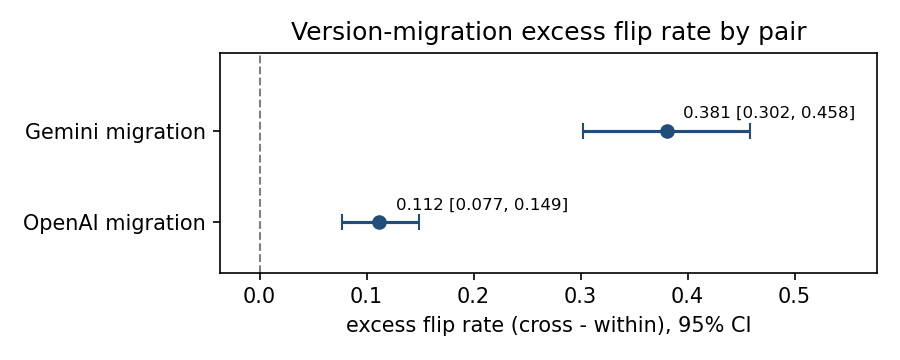
\includegraphics[width=\columnwidth]{fig1_excess_forest.png}
\caption{Excess flip rate (cross-version minus within-version noise floor) with 95\% CI for both migrations; both intervals exclude zero.}
\label{fig:forest}
\end{figure}

\subsection{Structural Decomposition of the Migration Effects}
Both migrations produce statistically significant excess flip rates, but the underlying structure of the decision change differs materially across providers. The prevalence--churn decomposition separates the gross cross-version flip rate into a marginal label-distribution shift and residual company-level churn (Fig.~\ref{fig:prev}).

For the OpenAI migration, the marginal shift is 0.095 and the churn component is 0.122, with a 95\% confidence interval for churn of $[0.083,\,0.161]$. Because churn exceeds the marginal shift, the OpenAI migration is primarily characterized by company-level reconsideration. A substantial share of firms move between categories in offsetting directions, so the aggregate label distribution changes less than the identities of the reclassified companies.

For the Gemini migration, the marginal shift is 0.319 and the churn component is 0.070, with a 95\% confidence interval for churn of $[0.029,\,0.120]$. Here, the marginal component is substantially larger than the churn component. The Gemini migration is therefore dominated by a portfolio-wide change in category prevalence rather than by offsetting company-specific reclassifications.

The difference can be summarized as
\begin{equation}
\text{OpenAI: } C > M, \qquad \text{Gemini: } M \gg C,
\end{equation}
where $C$ denotes churn and $M$ denotes marginal shift. The OpenAI successor primarily changes which companies receive particular credit-health labels, whereas the Gemini successor primarily changes the overall distribution of labels assigned across the evaluated portfolio.

Chance-corrected agreement statistics support the same distinction between the two migration pairs. For the OpenAI pair, Cohen's $\kappa$, Scott's $\pi$, and Gwet's AC1 are 0.60, 0.60, and 0.70, respectively. For the Gemini pair, the corresponding values are 0.33, 0.27, and 0.47. Although the absolute values differ across statistics because of their treatment of category prevalence, all three indicate materially greater cross-version consistency for the OpenAI migration than for the Gemini migration.

These results show that migration risk cannot be characterized by the excess flip rate alone. Two migrations may both produce material decision discontinuity while operating through different mechanisms: one mainly reclassifying individual companies, with the overall label distribution remaining relatively stable, and the other producing a broad shift in the portfolio-wide distribution of classifications.

\begin{figure}[t]
\centering
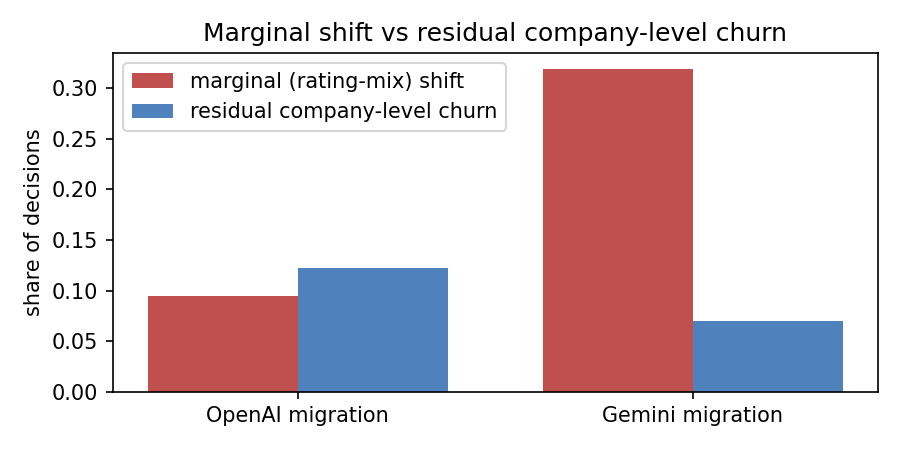
\includegraphics[width=\columnwidth]{fig2_prevalence.png}
\caption{Prevalence decomposition of the gross flip into a marginal (rating-mix) shift and residual company-level churn. OpenAI is churn-dominated; Gemini is marginal-dominated.}
\label{fig:prev}
\end{figure}

\subsection{Directional Drift Across Credit-Health Categories}
The two migrations shift credit-health classifications in opposite directions (Table~\ref{tab:mix}). The OpenAI successor shifts assessments toward more severe categories, whereas the Gemini successor shifts assessments toward the SAFE category.

For the OpenAI migration, the share of SAFE classifications decreases from 0.304 under the incumbent version to 0.209 under the successor. Over the same transition, the WATCH share increases from 0.588 to 0.636, and the DISTRESS share increases from 0.108 to 0.155:
\begin{equation}
\begin{aligned}
p_{\mathrm{SAFE}} &: 0.304 \rightarrow 0.209,\\
p_{\mathrm{WATCH}} &: 0.588 \rightarrow 0.636,\\
p_{\mathrm{DISTRESS}} &: 0.108 \rightarrow 0.155.
\end{aligned}
\end{equation}
The continuity-corrected McNemar test applied to the DISTRESS-versus-non-DISTRESS indicator yields
\begin{equation}
p \approx 6\times10^{-18},
\end{equation}
and the diagnostic is consistent with asymmetric movement toward DISTRESS.

The Gemini migration exhibits the opposite pattern. The SAFE share increases from 0.389 to 0.708, while WATCH decreases from 0.525 to 0.281 and DISTRESS decreases from 0.086 to 0.012:
\begin{equation}
\begin{aligned}
p_{\mathrm{SAFE}} &: 0.389 \rightarrow 0.708,\\
p_{\mathrm{WATCH}} &: 0.525 \rightarrow 0.281,\\
p_{\mathrm{DISTRESS}} &: 0.086 \rightarrow 0.012.
\end{aligned}
\end{equation}
For this migration, the corresponding McNemar test gives
\begin{equation}
p \approx 1.4\times10^{-59},
\end{equation}
and the diagnostic is consistent with asymmetric movement away from DISTRESS and toward less severe classifications.

The full $3\times3$ transition matrices reinforce these results (Fig.~\ref{fig:trans}). For OpenAI, off-diagonal mass is concentrated toward more severe categories, while for Gemini it is concentrated toward SAFE.

These findings show that version migration does not introduce a common directional bias across providers. The OpenAI successor produces systematically more conservative credit-health assessments, whereas the Gemini successor produces systematically more lenient assessments on the same task and evaluation period. The direction of migration-induced drift is therefore provider- and version-specific rather than predictable from migration alone.

\begin{table}[t]
\centering
\caption{Credit-label mix before/after each migration. OpenAI shifts toward DISTRESS; Gemini shifts sharply toward SAFE.}
\label{tab:mix}
\small
\begin{tabular}{@{}lccc@{}}
\toprule
Version & SAFE & WATCH & DISTRESS \\
\midrule
OpenAI $v_{\mathrm{old}}$ & 0.304 & 0.588 & 0.108 \\
OpenAI $v_{\mathrm{new}}$ & 0.209 & 0.636 & 0.155 \\
Gemini $v_{\mathrm{old}}$ & 0.389 & 0.525 & 0.086 \\
Gemini $v_{\mathrm{new}}$ & 0.708 & 0.281 & 0.012 \\
\bottomrule
\end{tabular}
\end{table}

\begin{figure}[t]
\centering
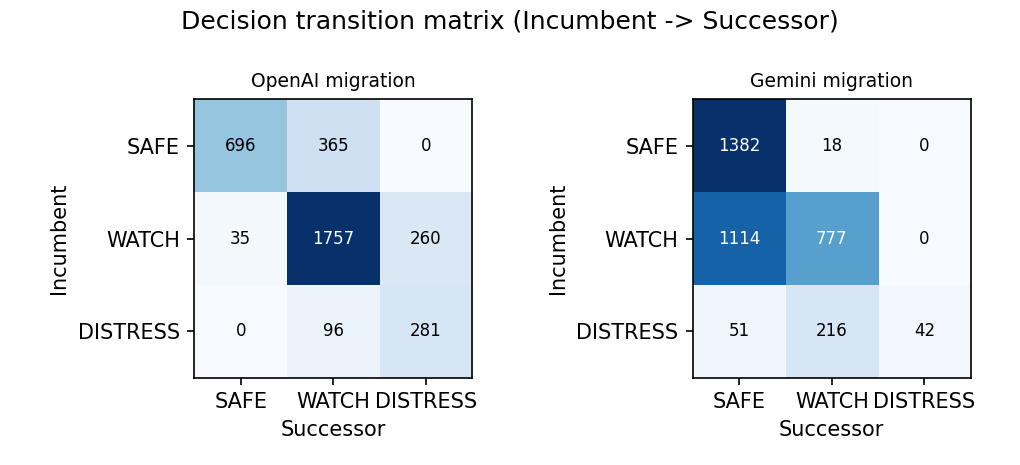
\includegraphics[width=0.72\textwidth]{fig3_transition.png}
\caption{Decision transition matrices ($v_{\mathrm{old}}\to v_{\mathrm{new}}$) for each migration. OpenAI's mass moves off the diagonal toward more-severe tiers; Gemini's moves sharply into SAFE.}
\label{fig:trans}
\end{figure}

\subsection{Robustness of Cross-Version Agreement}
The comparison between the two migrations is not sensitive to the choice of chance-corrected agreement statistic~\cite{cohen,scott,gwet}. For OpenAI,
\begin{equation}
\kappa=0.60,\qquad \pi=0.60,\qquad \mathrm{AC1}=0.70,
\end{equation}
whereas for Gemini,
\begin{equation}
\kappa=0.33,\qquad \pi=0.27,\qquad \mathrm{AC1}=0.47.
\end{equation}
Although the absolute values differ because the statistics treat category prevalence differently, all three produce the same ordering:
\begin{equation}
\text{OpenAI agreement}>\text{Gemini agreement}.
\end{equation}
The lower Gemini agreement is therefore not attributable solely to the prevalence sensitivity associated with Cohen's $\kappa$~\cite{feinstein}.

Migration effects are also larger among observations that are already unstable within the incumbent version. Relative to stable cells, the cross-version flip rate is higher by 0.330 for OpenAI and 0.250 for Gemini. This diagnostic pattern suggests that migration-induced changes are concentrated disproportionately near existing model decision boundaries, where classifications are already more sensitive to small changes in model behavior.

\subsection{Secondary Accuracy Analysis}
\label{sec:acc}
The primary analysis measures migration-induced decision instability independently of any reference label. As a secondary analysis, we evaluate whether the successor versions improve classification quality against the deterministic, rule-based Altman $Z''$-based reference categories. Because the three classes are imbalanced, performance is assessed using raw hit rate, balanced accuracy, and macro-F1 rather than raw accuracy alone.

For the OpenAI migration, classification performance changes as follows:
\begin{equation}
\begin{aligned}
\text{Hit rate} &: 0.539 \rightarrow 0.564,\\
\text{Balanced accuracy} &: 0.538 \rightarrow 0.570,\\
\text{Macro-F1} &: 0.517 \rightarrow 0.565.
\end{aligned}
\end{equation}
For the Gemini migration, performance declines:
\begin{equation}
\begin{aligned}
\text{Hit rate} &: 0.494 \rightarrow 0.425,\\
\text{Balanced accuracy} &: 0.488 \rightarrow 0.408,\\
\text{Macro-F1} &: 0.463 \rightarrow 0.325.
\end{aligned}
\end{equation}
The OpenAI successor produces modest numerical improvements, but the migration does not reliably improve accuracy on the specific observations whose labels change. Conditional on a cross-version flip, the estimated accuracy change is $+0.124$, with a 95\% confidence interval of $[-0.164,\,0.418]$.

For Gemini, the successor's large shift toward SAFE is accompanied by lower class-balanced performance. The flip-conditional accuracy change is $-0.179$, with a 95\% confidence interval of $[-0.380,\,0.030]$. The interval includes zero; the accompanying lower balanced accuracy and macro-F1 are consistent with the distributional shift toward SAFE providing no compensating classification improvement.

The sector-restricted analysis excludes Financials and Real Estate, for which the Altman $Z''$ reference model is less suitable. The principal pattern remains: raw hit rate changes from 0.590 to 0.562 for the OpenAI migration and from 0.553 to 0.491 for the Gemini migration.

These results show that substantial migration-induced decision changes do not necessarily correspond to improved classification quality. The OpenAI successor shows modest numerical improvement in aggregate metrics, whereas the Gemini successor shows lower class-balanced performance; neither migration shows clear improvement among the observations whose labels change. The accuracy analysis is secondary and does not affect the primary conclusion that both migrations produce cross-version disagreement well above the within-version noise floor.

\subsection{Temperature Sensitivity}
A supplementary temperature analysis evaluates whether the migration effect depends on the primary decoding setting of $T=0$. Both migration pairs are re-estimated on a smaller stratified subgrid at $T\in\{0,0.7,1.0\}$.

For OpenAI, the estimated excess flip rates are 0.153, 0.167, and 0.208 at $T=0$, $0.7$, and $1.0$, respectively (Table~\ref{tab:temp}). For Gemini, the corresponding estimates are 0.222, 0.306, and 0.389. The estimated effect remains positive for both migration pairs at every tested temperature.

The confidence intervals are wide because the robustness grid contains only 24 company--date cells. In particular, the lower bound for Gemini at $T=0$ reaches zero. The temperature analysis should therefore be interpreted as evidence that the direction of the migration effect is preserved across the tested settings, not as an independently powered estimate of its magnitude.

The full-grid $T=0$ analysis remains the primary result. The smaller temperature sweep provides supporting evidence that the observed version discontinuity is not limited to a single decoding temperature.

\begin{table}[t]
\centering
\caption{Temperature-sensitivity robustness (excess flip rate with 95\% CI, $8\times3$ subgrid).}
\label{tab:temp}
\small
\begin{tabular}{@{}lcc@{}}
\toprule
$T$ & OpenAI & Gemini \\
\midrule
0.0 & 0.153 [.042,.278] & 0.222 [.000,.500] \\
0.7 & 0.167 [.056,.292] & 0.306 [.111,.500] \\
1.0 & 0.208 [.069,.361] & 0.389 [.167,.611] \\
\bottomrule
\end{tabular}
\end{table}

\section{Discussion}
\label{sec:disc}
Vendor-driven model-version migration leads to materially different categorical financial decisions even when the prompt, inputs, inference settings, and downstream workflow remain fixed. After accounting for within-version variability, the noise-adjusted excess cross-version disagreement is approximately 11 percentage points for the OpenAI migration and approximately 38 percentage points for the Gemini migration. The two migrations also differ structurally: OpenAI is primarily churn-dominated and shifts assessments toward greater severity, whereas Gemini is primarily prevalence-dominated and shifts the portfolio toward SAFE. Migration behavior therefore cannot be assumed to be uniformly conservative, permissive, or performance-enhancing.

The prevalence--churn decomposition has direct operational significance. A prevalence-dominated migration changes the overall distribution of ratings and may affect portfolio limits, escalation volumes, and review capacity. A churn-dominated migration may leave the aggregate rating mix comparatively stable while changing which individual companies are identified as risky. The secondary accuracy analysis further shows that decision turnover does not necessarily produce better classification quality. The OpenAI successor exhibits modest numerical improvement without reliable improvement among changed observations, while the Gemini successor exhibits lower balanced accuracy and macro-F1. Vendor migration should therefore be treated as a model change requiring validation rather than as an automatic upgrade.

The Altman $Z''$-based label serves only as a deterministic reference proxy for the secondary outcome analysis~\cite{altman_em}; the primary instability, agreement, churn, and directional-drift results depend solely on paired model outputs. More broadly, the findings establish a deployment-level mechanism through which systems using the same vendor version could experience a common behavioral change when migrated to the same successor~\cite{kim,monoculture,esrb}. The study does not measure cross-institutional adoption, realized losses, or market-level systemic effects. It demonstrates that the shared-update mechanism exists and can be measured, motivating the governance control developed in Section~\ref{sec:gov}.

\section{Governance: SR 11-7, SR 26-2, and a Pre-Migration Control}
\label{sec:gov}
SR 11-7 historically organized U.S. model-risk governance around independent validation, effective challenge, ongoing monitoring, change management, and institutional responsibility for third-party models~\cite{sr117}. Its lifecycle generally assumes that an institution can identify when a model changes and evaluate the modified model before production use. Vendor-managed foundation models weaken this assumption because the provider determines the successor version and deprecation schedule, while the surrounding prompt, application, and API interface may remain substantially unchanged. A migration can therefore substitute one decision function for another without appearing as a conventional redevelopment event.

The governance gap is sharper under the current framework. SR 26-2, which replaced SR 11-7 in April 2026, expressly excludes generative and agentic AI from its scope because of their novelty and rapid evolution~\cite{sr2602}. The class of systems evaluated in this study therefore falls outside the revised guidance. Moreover, although SR 26-2 strengthens the treatment of concentration and dependency within an institution's model portfolio, it does not address correlated behavioral changes across institutions or deployments that depend on the same vendor version. The resulting gap is twofold: generative-AI systems are excluded from the revised framework, and the cross-deployment consequences of a common vendor update are not directly governed.

The empirical results connect to three established governance concerns summarized in Table~\ref{tab:gov}. First, a vendor migration may constitute a material behavioral change even when no internal code or prompt changes. Second, limited deprecation notice may restrict the pre-production comparison needed for effective challenge. Third, recording only the provider or model-family name is insufficient when exact snapshots exhibit materially different behavior. Exact version identifiers should therefore be maintained as governed model artifacts, and a version change should trigger formal testing, documentation, and approval.

Shared reliance on the same hosted version also creates a concentration channel beyond the model inventory of a single institution~\cite{esrb}. Multiple deployments may encounter the same provider-initiated change at approximately the same time. This study does not establish realized cross-institutional losses or systemic instability; it identifies the decision-level mechanism through which a common migration could produce correlated movement across deployments pinned to the shared version.

We propose a pre-migration parallel run conducted before production cutover. The institution applies the incumbent and successor versions to the same frozen, representative inputs using identical prompts, inference settings, and downstream decision rules. The control should estimate
\begin{equation}
F_{\mathrm{excess}} = F_{\mathrm{cross}} - F_{\mathrm{noise}},
\end{equation}
together with the prevalence--churn decomposition and a directional-drift test. Where a defensible reference outcome exists, comparative performance should be evaluated as a secondary validation axis.

Cutover criteria should be specified before testing. Excess disagreement above an institution-defined materiality threshold, material directional drift, or disproportionate movement among high-risk cases should trigger expanded validation and documented approval rather than automatic deployment. Institutions should also inventory exact snapshot identifiers, seek advance deprecation notice, preserve access to the incumbent throughout the validation window, and retain frozen incumbent outputs as a challenger benchmark. The resulting parallel-run package provides evidence for monitoring, effective challenge, and change approval. This proposal is a practitioner-oriented control interpretation rather than authoritative supervisory guidance.

\begin{table}[t]
\centering
\caption{Mapping vendor version migration to SR 11-7 provisions and the proposed control.}
\label{tab:gov}
\small
\begin{tabular}{@{}p{0.30\textwidth}p{0.37\textwidth}p{0.27\textwidth}@{}}
\toprule
SR 11-7 provision & How version migration breaks it & Proposed control \\
\midrule
Vendor/third-party responsibility \& contingency planning & Anticipates vendor-model \emph{loss}, not silent behavioral \emph{replacement} on the vendor's schedule & Inventory the exact version string; pin the incumbent through validation \\
Ongoing monitoring; accelerate review on material model change & The change is exogenous and silent (API surface unchanged), so it may never trigger the review it warrants & Pre-migration parallel run detects the change and quantifies its materiality \\
Effective challenge; validation before use & Forced deprecation with limited notice removes the pre-change testable window & Parallel-run gate provides challenge and validation evidence before cutover \\
Model inventory, change control, documentation & Frozen documentation undermined by a model that changes underneath it & Treat version-as-artifact; hash-pin the snapshot as the object of record \\
Aggregate (institution-level) model risk & Not contemplated as correlated \emph{across} institutions via a shared vendor update & Systemic gap; flagged for supervisory attention \\
\bottomrule
\end{tabular}
\end{table}

\section{Threats to Validity}
\noindent\textbf{Endpoint variability.} Hosted LLM endpoints can remain stochastic even when temperature is set to zero and a seed is supplied. The study therefore does not assume deterministic model behavior. Instead, repeated within-version calls estimate residual variability, which is subtracted from the cross-version flip rate in the primary endpoint.

\noindent\textbf{Reference-label limitations.} Altman $Z''$ provides a deterministic, rule-based classification reference, but it is a proxy for realized credit outcomes and is not equally suitable for all sectors. It is therefore used only for the secondary accuracy analysis. The primary excess-flip, agreement, prevalence, churn, and directional-drift results do not depend on the reference labels.

\noindent\textbf{Thin DISTRESS stratum.} DISTRESS classifications constitute a relatively small share of the evaluated observations, so estimates involving movement into or out of the most severe category are based on fewer cells than the SAFE and WATCH comparisons. Estimates involving the DISTRESS class should therefore be interpreted with caution. This does not affect the primary migration-instability result, which does not depend on the prevalence of the Altman reference label.

\noindent\textbf{Task and prompt scope.} The experiment evaluates one structured credit-health classification task using a single prompt family and standardized financial inputs. The measured effect sizes may differ for other prompts, domains, and input formats. The controlled design improves causal isolation and reproducibility but does not reproduce the full complexity of production workflows involving unstructured filings, retrieval systems, human review, or downstream automation.

\noindent\textbf{Provider and migration-pair scope.} Two migration pairs establish that material decision discontinuity can occur and that its direction and structure may differ across providers. They do not characterize the distribution of migration effects across the broader model ecosystem. Additional migrations and tasks are required before making claims about typical effect size, provider ranking, or model-family behavior.

\noindent\textbf{Systemic-risk interpretation.} The study measures synchronized decision changes at the deployment level, not realized cross-institutional losses or market instability. The results identify a mechanism through which deployments sharing the same model version could experience correlated movement. Whether this mechanism produces material system-wide effects depends on adoption concentration, institutional implementation, downstream controls, and economic exposure, none of which are observed here.

\noindent\textbf{Single collection window.} Confirmatory responses were collected once from exact model snapshots. Provider-side changes occurring during the collection period cannot be completely ruled out or averaged across repeated collection windows. The frozen call-level dataset is therefore the empirical object of record, and the findings apply to the evaluated snapshots and collection period.

\section{Conclusion}
Vendor-managed LLM migrations are associated with material decision discontinuities within otherwise unchanged financial workflows. After accounting for within-version variability, the noise-adjusted excess cross-version disagreement is 11.2 percentage points for the OpenAI migration and 38.1 percentage points for the Gemini migration. OpenAI primarily reclassifies individual companies and shifts decisions toward greater severity; Gemini primarily changes the portfolio-wide label distribution and shifts decisions toward SAFE. Neither migration shows clear improvement among observations whose labels change; the Gemini successor also shows lower aggregate class-balanced performance.

The study contributes a measurement framework that separates cross-version disagreement from ordinary endpoint variability and distinguishes distributional movement from company-level churn. These measures support a pre-migration parallel-run control through which institutions can evaluate successor models before production cutover.

The evidence is limited to two migration pairs, one structured classification task, and one prompt family. It does not estimate typical migration effects or realized market-level consequences. It nevertheless demonstrates a deployment-level mechanism through which systems using a shared vendor version may experience a common behavioral shock when that version is replaced.

Exact model versions should therefore be treated as governed artifacts, and vendor migrations should trigger documented testing, effective challenge, and change approval. The frozen, preregistered analytical package provides a reproducible basis for conducting and auditing such evaluations without assuming that future proprietary-endpoint calls will reproduce the archived responses.

\section*{Data and Code Availability}
To support reproduction, we release: (i)~the immutable, read-only,
SHA-256-stamped raw dataset (\texttt{data/raw/}), containing 14{,}400 logged
calls with the per-call model, seed, prompt hash, timestamp, token usage, cost,
and raw response; (ii)~the pre-registration materials and the cryptographic
freeze receipt; (iii)~the deterministic, seeded analysis pipeline that
regenerates every table and figure in this paper, together with a replication
check; and (iv)~the capture and monitoring harness (the pre-migration
parallel-run metric). Code and data are available at
\url{https://github.com/samirrc2/version-migration-shock}.
A Code Ocean compute capsule enabling keys-free reproduction is available at
\url{https://doi.org/10.24433/CO.2874343.v1}
(DOI:~\texttt{10.24433/CO.2874343.v1}).
The dataset SHA-256 hashes and analysis commit hash are recorded in the
supplementary manifest.

\section*{Acknowledgment}
The authors thank colleagues and reviewers for feedback.

\section*{Use of Generative AI}
The authors acknowledge the use of artificial intelligence (AI) tools for the
preparation of this manuscript. Specifically, OpenAI's ChatGPT (GPT-5, 2025)
and Anthropic's Claude were employed to support tasks such as text drafting,
language polishing, formatting guidance, and code review. All outputs from
these tools were critically examined, verified, and edited by the authors to
ensure accuracy and originality.

\begin{thebibliography}{99}
\small
\bibitem{muscle} J. Zhang \emph{et al.}, ``MUSCLE: A Model Update Strategy for Compatible LLM Evolution,'' arXiv:2407.09435, 2024. [Online]. Available: \url{https://arxiv.org/abs/2407.09435}
\bibitem{underspec} C. Yang, Y. Shi, Q. Ma, M. X. Liu, C. K\"astner, and T. Wu, ``What Prompts Don't Say: Understanding and Managing Underspecification in LLM Prompts,'' arXiv:2505.13360, 2025. [Online]. Available: \url{https://arxiv.org/abs/2505.13360}
\bibitem{kim} J. Kim \emph{et al.}, ``Correlated Errors in Large Language Models,'' arXiv:2506.07962, 2025. [Online]. Available: \url{https://arxiv.org/abs/2506.07962}
\bibitem{systemic} J. Dan\'ielsson, R. Macrae, and A. Uthemann, ``Artificial intelligence and systemic risk,'' \emph{Journal of Banking \& Finance}, vol.~140, art.~106290, 2022, doi:10.1016/j.jbankfin.2021.106290.
\bibitem{homog} R. Bommasani, K. A. Creel, A. Kumar, D. Jurafsky, and P. Liang, ``Picking on the same person: Does algorithmic monoculture lead to outcome homogenization?'' in \emph{Advances in Neural Information Processing Systems (NeurIPS)}, vol.~35, 2022. [Online]. Available: \url{https://arxiv.org/abs/2211.13972}
\bibitem{esrb} S.\ Cecchetti, R.\ L.\ Lumsdaine, T.\ Peltonen, and A.\ S\'anchez Serrano, ``Artificial Intelligence and Systemic Risk,'' Reports of the ESRB Advisory Scientific Committee, No.~16, Dec.\ 2025.
\bibitem{sr117} Board of Governors of the Federal Reserve System and OCC, ``SR 11-7: Guidance on Model Risk Management,'' 2011.
\bibitem{sr2602} Board of Governors of the Federal Reserve System, OCC, and FDIC, ``SR 26-2: Revised Guidance on Model Risk Management,'' April 17, 2026 (supersedes SR 11-7); OCC Bulletin 2026-13.
\bibitem{mrm} National Institute of Standards and Technology, ``Artificial Intelligence Risk Management Framework: Generative AI Profile,'' NIST Trustworthy and Responsible AI, NIST AI 600-1, Jul.\ 2024, doi:10.6028/NIST.AI.600-1.
\bibitem{gwet} K. L. Gwet, ``Computing inter-rater reliability and its variance in the presence of high agreement,'' British J.\ Math.\ Stat.\ Psychology, vol.~61, pp.~29--48, 2008.
\bibitem{altman} E. I. Altman, ``Financial Ratios, Discriminant Analysis and the Prediction of Corporate Bankruptcy,'' Journal of Finance, vol.~23, no.~4, pp.~589--609, 1968.
\bibitem{altman_em} E. I. Altman, ``An Emerging Market Credit Scoring System for Corporate Bonds,'' Emerging Markets Review, vol.~6, no.~4, pp.~311--323, 2005 (see also Altman, Hartzell, and Peck, 1995), which defines the $Z''$ model and its non-manufacturer / emerging-market cutoffs (2.6 / 1.1).
\bibitem{cohen} J. Cohen, ``A coefficient of agreement for nominal scales,'' \emph{Educational and Psychological Measurement}, vol.~20, no.~1, pp.~37--46, 1960.
\bibitem{scott} W. A. Scott, ``Reliability of content analysis: The case of nominal scale coding,'' \emph{Public Opinion Quarterly}, vol.~19, no.~3, pp.~321--325, 1955.
\bibitem{fleiss} J. L. Fleiss, ``Measuring nominal scale agreement among many raters,'' \emph{Psychological Bulletin}, vol.~76, no.~5, pp.~378--382, 1971.
\bibitem{feinstein} A. R. Feinstein and D. V. Cicchetti, ``High agreement but low kappa: I. The problems of two paradoxes,'' \emph{Journal of Clinical Epidemiology}, vol.~43, no.~6, pp.~543--549, 1990.
\bibitem{mcnemar} Q. McNemar, ``Note on the sampling error of the difference between correlated proportions or percentages,'' \emph{Psychometrika}, vol.~12, no.~2, pp.~153--157, 1947.
\bibitem{efron} B. Efron, ``Bootstrap methods: Another look at the jackknife,'' \emph{Annals of Statistics}, vol.~7, no.~1, pp.~1--26, 1979.
\bibitem{bommasani} R. Bommasani \emph{et al.}, ``On the Opportunities and Risks of Foundation Models,'' arXiv:2108.07258, 2021. [Online]. Available: \url{https://arxiv.org/abs/2108.07258}
\bibitem{helm} P. Liang \emph{et al.}, ``Holistic Evaluation of Language Models,'' \emph{Trans.\ Machine Learning Research}, 2023; arXiv:2211.09110.
\bibitem{bloomberggpt} S. Wu \emph{et al.}, ``BloombergGPT: A Large Language Model for Finance,'' arXiv:2303.17564, 2023. [Online]. Available: \url{https://arxiv.org/abs/2303.17564}
\bibitem{finbert} D. Araci, ``FinBERT: Financial Sentiment Analysis with Pre-trained Language Models,'' arXiv:1908.10063, 2019. [Online]. Available: \url{https://arxiv.org/abs/1908.10063}
\bibitem{monoculture} J. Kleinberg and M. Raghavan, ``Algorithmic monoculture and social welfare,'' \emph{Proc.\ Nat.\ Acad.\ Sci.}, vol.~118, no.~22, e2018340118, 2021.
\bibitem{wei} J. Wei \emph{et al.}, ``Emergent Abilities of Large Language Models,'' \emph{Trans.\ Machine Learning Research}, 2022; arXiv:2206.07682.
\bibitem{gama} J. Gama, I. \v{Z}liobait\.{e}, A. Bifet, M. Pechenizkiy, and A. Bouchachia, ``A survey on concept drift adaptation,'' \emph{ACM Computing Surveys}, vol.~46, no.~4, pp.~1--37, 2014.
\bibitem{pctrain} S. Yan \emph{et al.}, ``Positive-congruent training: Towards regression-free model updates,'' in \emph{Proc.\ IEEE/CVF Conf.\ Computer Vision and Pattern Recognition (CVPR)}, 2021, pp.~14299--14308.
\bibitem{sclar} M. Sclar, Y. Choi, Y. Tsvetkov, and A. Suhr, ``Quantifying Language Models' Sensitivity to Spurious Features in Prompt Design,'' in \emph{Proc.\ Int.\ Conf.\ Learning Representations (ICLR)}, 2024; arXiv:2310.11324.
\bibitem{fsb} Financial Stability Board, ``Artificial Intelligence and Machine Learning in Financial Services,'' Nov.\ 2017.
\bibitem{gpt4} OpenAI, ``GPT-4 Technical Report,'' arXiv:2303.08774, 2023. [Online]. Available: \url{https://arxiv.org/abs/2303.08774}
\bibitem{nosek} B. A. Nosek, C. R. Ebersole, A. C. DeHaven, and D. T. Mellor, ``The preregistration revolution,'' \emph{Proc.\ Nat.\ Acad.\ Sci.}, vol.~115, no.~11, pp.~2600--2606, 2018.
\bibitem{simmons} J. P. Simmons, L. D. Nelson, and U. Simonsohn, ``False-positive psychology: Undisclosed flexibility in data collection and analysis allows presenting anything as significant,'' \emph{Psychological Science}, vol.~22, no.~11, pp.~1359--1366, 2011.
\bibitem{pineau} J. Pineau \emph{et al.}, ``Improving reproducibility in machine learning research (a report from the NeurIPS 2019 reproducibility program),'' \emph{Journal of Machine Learning Research}, vol.~22, no.~164, pp.~1--20, 2021.
\bibitem{openai_dep} OpenAI, ``Deprecations,'' OpenAI API Documentation, 2026. [Online]. Available: \url{https://developers.openai.com/api/docs/deprecations} (accessed Jul.~4, 2026).
\bibitem{google_dep} Google, ``Gemini deprecations,'' Google AI for Developers, 2026. [Online]. Available: \url{https://ai.google.dev/gemini-api/docs/deprecations} (accessed Jul.~4, 2026).
\end{thebibliography}

\section*{Author Biographies}
\noindent\textbf{Samir Chincholikar.} 
received the B.E. degree from the University of Mumbai, India, in 2013, the
M.B.A. degree in finance from the Jamnalal Bajaj Institute of Management
Studies, University of Mumbai, in 2016, and the M.S. degree in financial
engineering from the University of Illinois Urbana-Champaign, Urbana, IL, USA,
in 2019. He has over a decade of professional experience in quantitative risk
analytics and machine learning in the financial services industry. His research
interests include large language models, multi-agent systems, the use of AI to
automate engineering workflows, machine learning evaluation, and reproducible
empirical methods in computational finance.




\medskip\noindent\textbf{Robin Chawla.} 
received the B.Tech. degree in computer science and engineering from the Indian
Institute of Technology (BHU), Varanasi, India. He has about eight years of
professional experience as a software engineer at a proprietary trading firm,
focused on low-latency systems, performance-oriented software, and the use of
AI to automate engineering workflows. His research interests include large
language models, multi-agent systems, machine learning for engineering
workflows and automation, and reproducible evaluation of generative AI
for decision-making.




\end{document}
